\documentclass[ignorenonframetext,]{beamer}
\setbeamertemplate{caption}[numbered]
\setbeamertemplate{caption label separator}{: }
\setbeamercolor{caption name}{fg=normal text.fg}
\beamertemplatenavigationsymbolsempty
\usepackage{lmodern}
\usepackage{amssymb,amsmath}
\usepackage{ifxetex,ifluatex}
\usepackage{fixltx2e} % provides \textsubscript
\ifnum 0\ifxetex 1\fi\ifluatex 1\fi=0 % if pdftex
  \usepackage[T1]{fontenc}
  \usepackage[utf8]{inputenc}
\else % if luatex or xelatex
  \ifxetex
    \usepackage{mathspec}
  \else
    \usepackage{fontspec}
  \fi
  \defaultfontfeatures{Ligatures=TeX,Scale=MatchLowercase}
\fi
\usetheme[]{Warsaw}
% use upquote if available, for straight quotes in verbatim environments
\IfFileExists{upquote.sty}{\usepackage{upquote}}{}
% use microtype if available
\IfFileExists{microtype.sty}{%
\usepackage{microtype}
\UseMicrotypeSet[protrusion]{basicmath} % disable protrusion for tt fonts
}{}
\newif\ifbibliography
\hypersetup{
            pdftitle={Glaucoma Structural Progression},
            pdfauthor={Davide Burba, Matteo Muffo},
            pdfborder={0 0 0},
            breaklinks=true}
\urlstyle{same}  % don't use monospace font for urls
\usepackage{graphicx,grffile}
\makeatletter
\def\maxwidth{\ifdim\Gin@nat@width>\linewidth\linewidth\else\Gin@nat@width\fi}
\def\maxheight{\ifdim\Gin@nat@height>\textheight0.8\textheight\else\Gin@nat@height\fi}
\makeatother
% Scale images if necessary, so that they will not overflow the page
% margins by default, and it is still possible to overwrite the defaults
% using explicit options in \includegraphics[width, height, ...]{}
\setkeys{Gin}{width=\maxwidth,height=\maxheight,keepaspectratio}

% Prevent slide breaks in the middle of a paragraph:
\widowpenalties 1 10000
\raggedbottom

\AtBeginPart{
  \let\insertpartnumber\relax
  \let\partname\relax
  \frame{\partpage}
}
\AtBeginSection{
  \ifbibliography
  \else
    \let\insertsectionnumber\relax
    \let\sectionname\relax
    \frame{\sectionpage}
  \fi
}
\AtBeginSubsection{
  \let\insertsubsectionnumber\relax
  \let\subsectionname\relax
  \frame{\subsectionpage}
}

\setlength{\parindent}{0pt}
\setlength{\parskip}{6pt plus 2pt minus 1pt}
\setlength{\emergencystretch}{3em}  % prevent overfull lines
\providecommand{\tightlist}{%
  \setlength{\itemsep}{0pt}\setlength{\parskip}{0pt}}
\setcounter{secnumdepth}{0}

\title{Glaucoma Structural Progression}
\author{Davide Burba, Matteo Muffo}
\date{December 1, 2017}

\begin{document}
\frame{\titlepage}

\begin{frame}{IMPORTAZIONE DATI}

\textcolor{red}{PROVA}

\end{frame}

\begin{frame}{EXPLORATORY ANALYSIS}

\begin{itemize}
\tightlist
\item
  Number of visits per patient
\end{itemize}

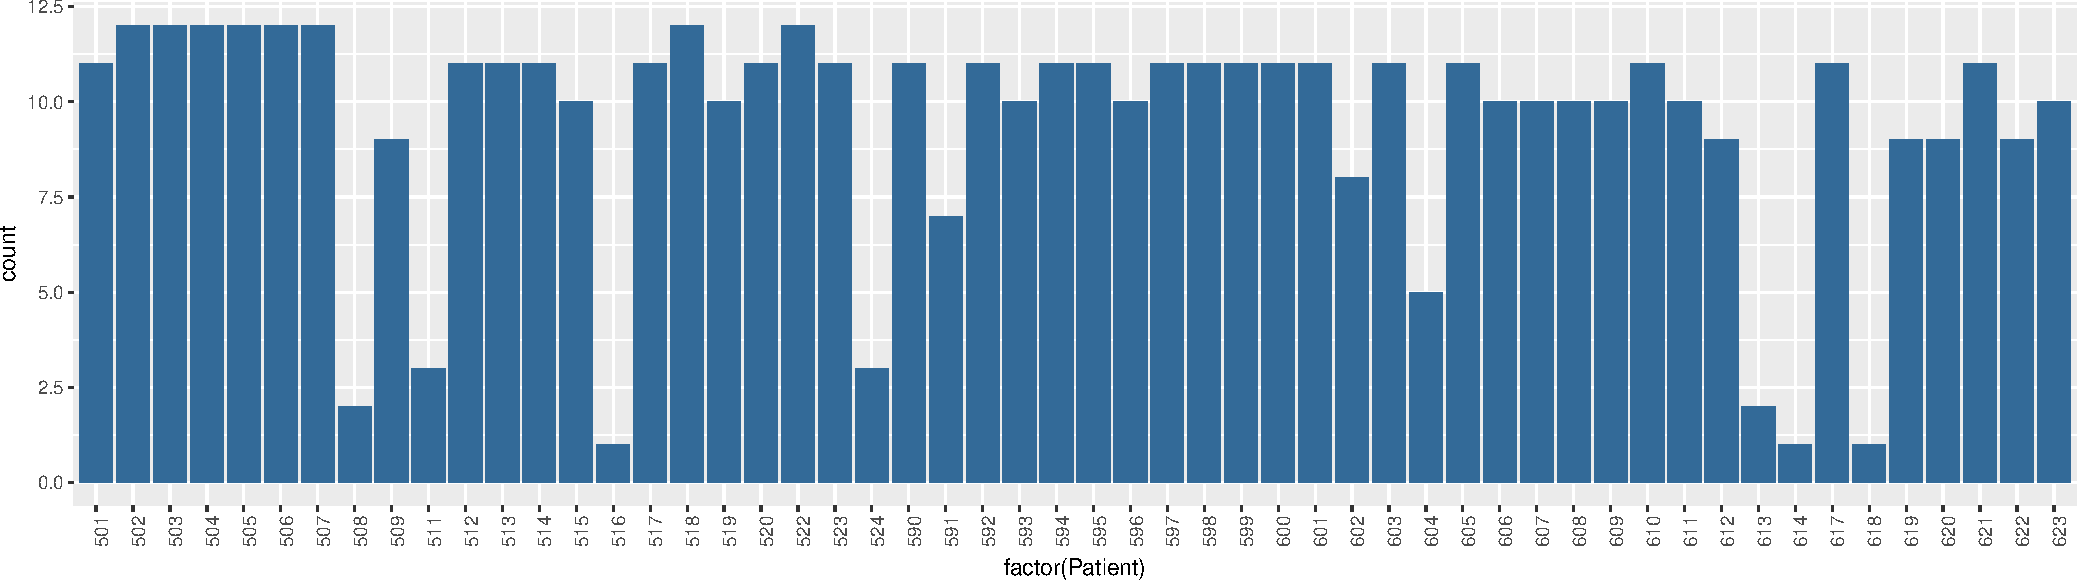
\includegraphics{analisi_exp_markdown_files/figure-beamer/unnamed-chunk-2-1.pdf}

\begin{itemize}
\tightlist
\item
  Mean number of observations: 9.2
\item
  0.25 quantile: 9
\item
  0.50 quantile: 11
\item
  0.75 quantile: 11
\end{itemize}

\end{frame}

\begin{frame}{}

\begin{itemize}
\tightlist
\item
  female vs male
\end{itemize}

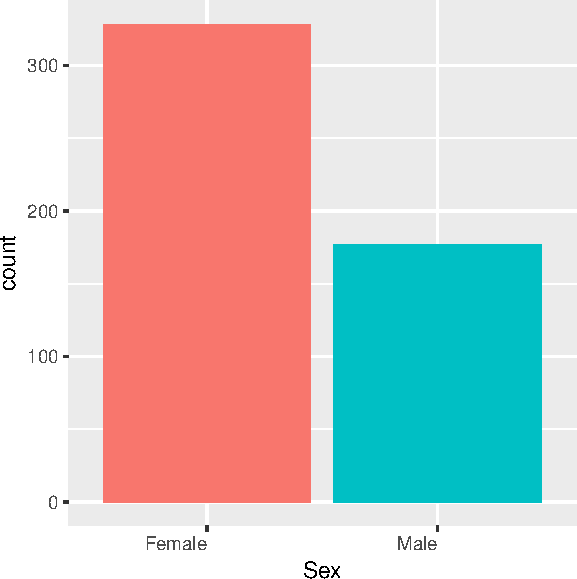
\includegraphics{analisi_exp_markdown_files/figure-beamer/unnamed-chunk-4-1.pdf}

\end{frame}

\begin{frame}{}

\begin{itemize}
\tightlist
\item
  type of glaucoma
\end{itemize}

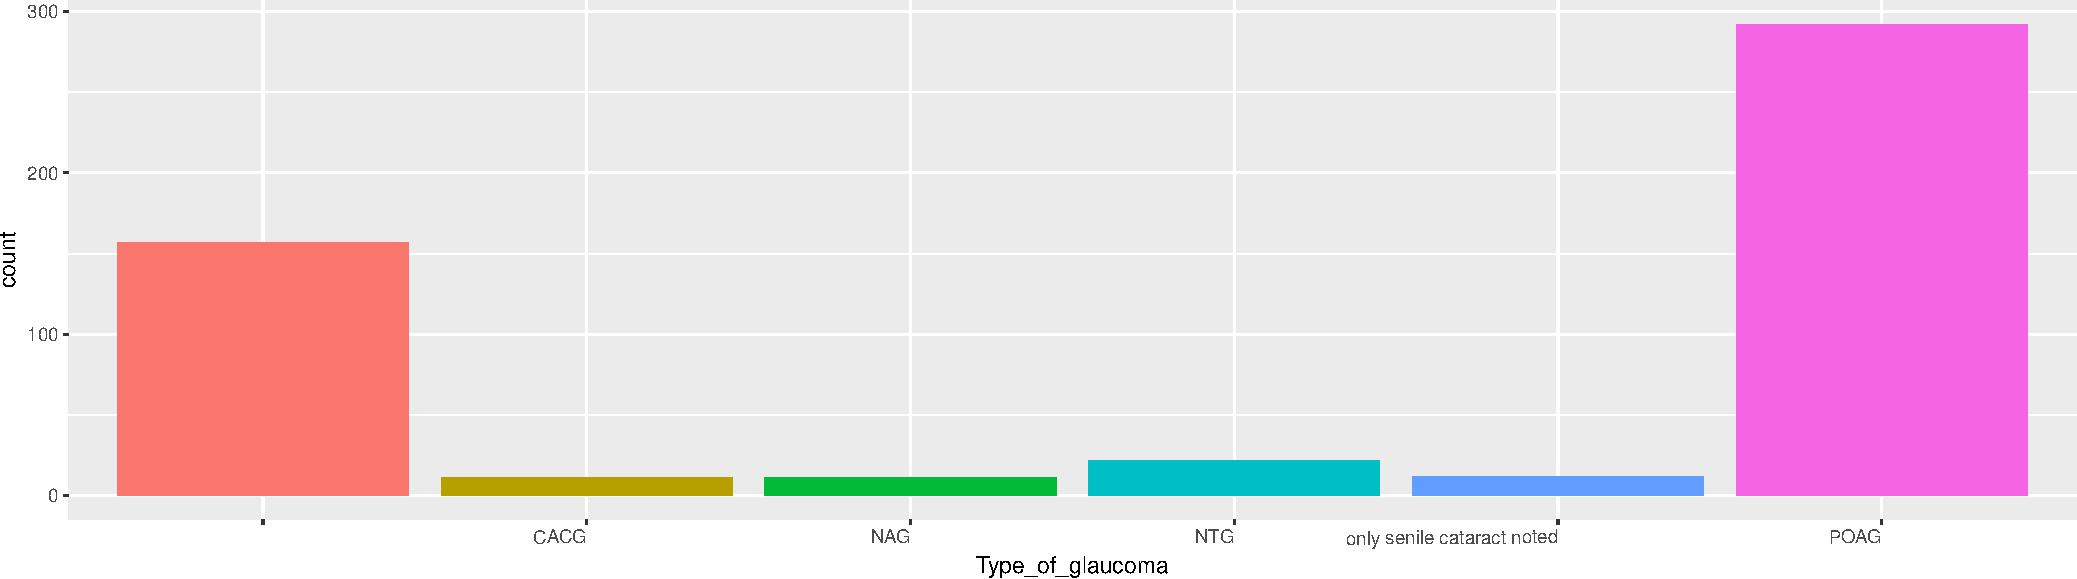
\includegraphics{analisi_exp_markdown_files/figure-beamer/unnamed-chunk-5-1.pdf}

\end{frame}

\begin{frame}{A UNIQUE PATIENT}

Some variables:

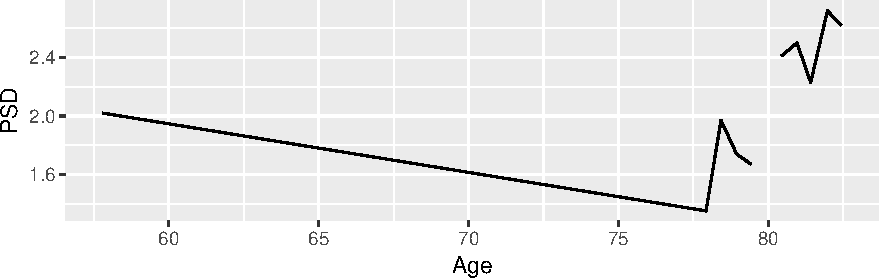
\includegraphics{analisi_exp_markdown_files/figure-beamer/unnamed-chunk-8-1.pdf}

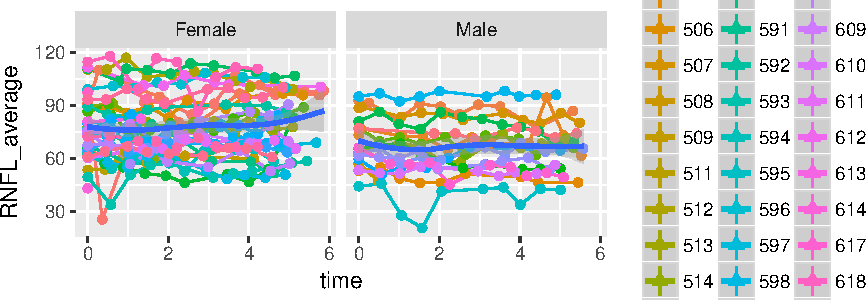
\includegraphics{analisi_exp_markdown_files/figure-beamer/unnamed-chunk-9-1.pdf}

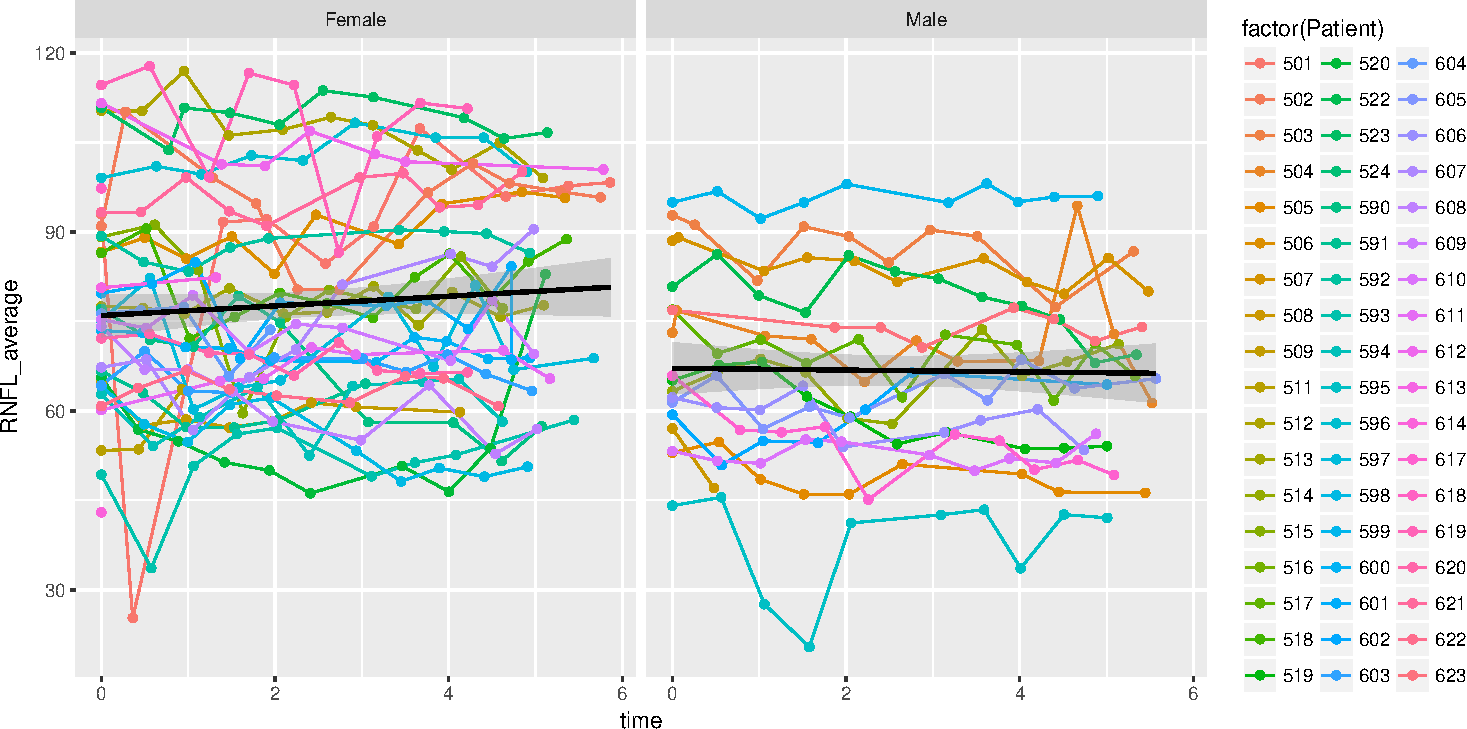
\includegraphics{analisi_exp_markdown_files/figure-beamer/unnamed-chunk-10-1.pdf}

\end{frame}

\begin{frame}{}

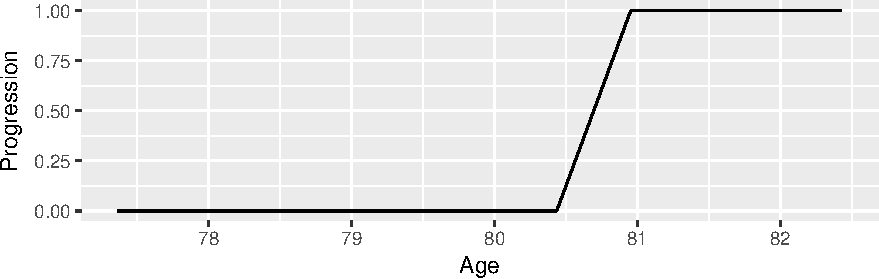
\includegraphics{analisi_exp_markdown_files/figure-beamer/unnamed-chunk-11-1.pdf}

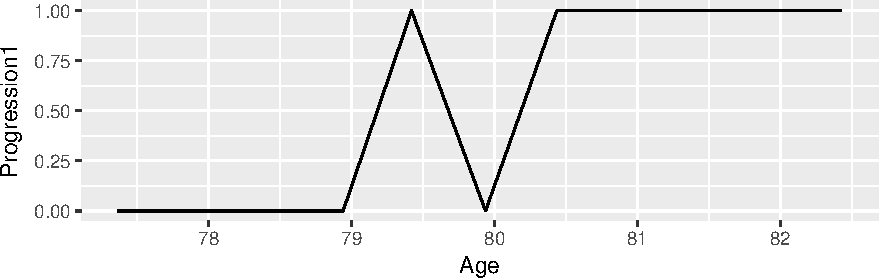
\includegraphics{analisi_exp_markdown_files/figure-beamer/unnamed-chunk-12-1.pdf}

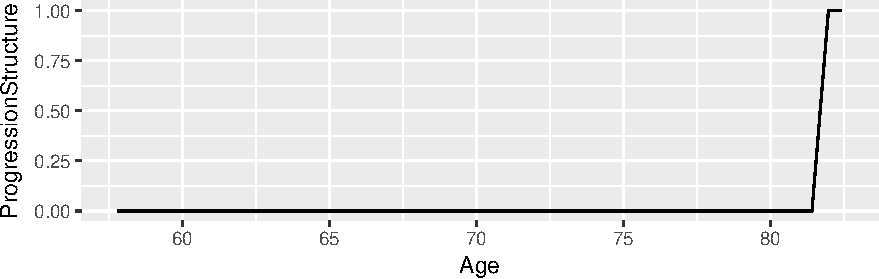
\includegraphics{analisi_exp_markdown_files/figure-beamer/unnamed-chunk-13-1.pdf}

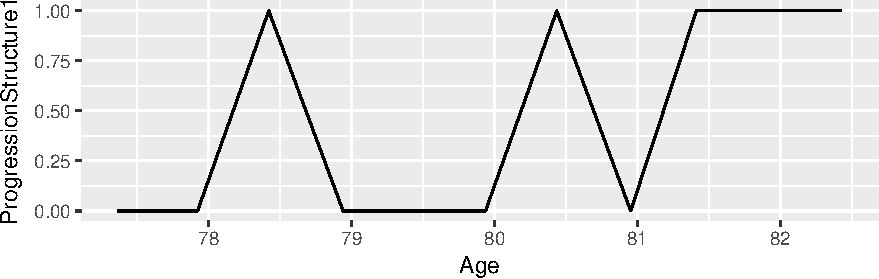
\includegraphics{analisi_exp_markdown_files/figure-beamer/unnamed-chunk-14-1.pdf}

\end{frame}

\begin{frame}{ALL THE PATIENTS}

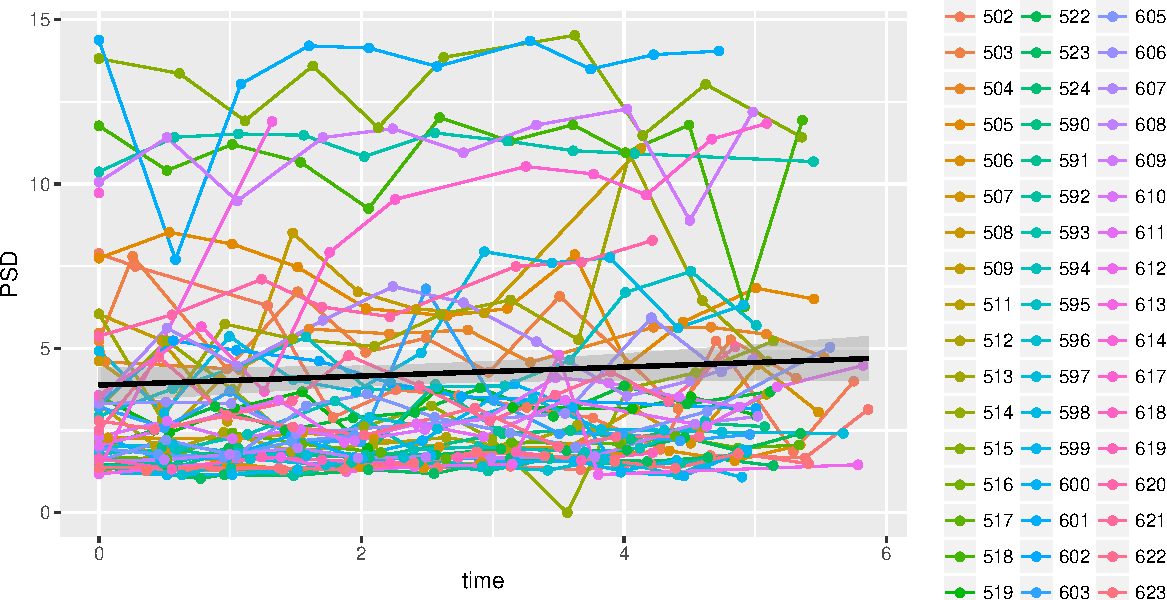
\includegraphics{analisi_exp_markdown_files/figure-beamer/unnamed-chunk-15-1.pdf}

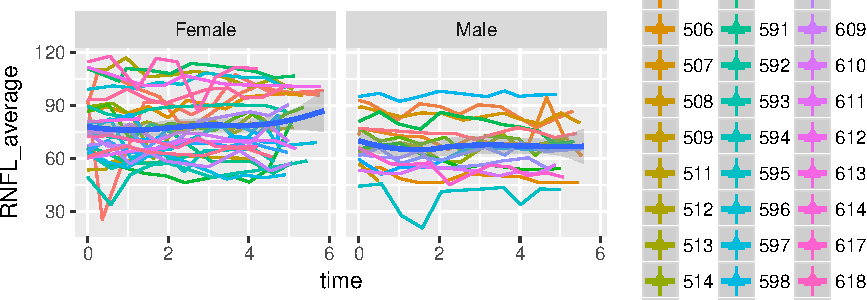
\includegraphics{analisi_exp_markdown_files/figure-beamer/unnamed-chunk-16-1.pdf}

\end{frame}

\begin{frame}{TODO:}

\begin{itemize}
\tightlist
\item
  Plot decenti di tutti i pazienti
\item
  Plot e analisi esplorativa altre variabili
\item
  Riempire dati mancanti
\end{itemize}

\end{frame}

\end{document}
